\subsection*{More about Venn Diagrams} \label{ss:venn3}
In \typeu Activity~\ref*{PA:venn}, we learned how to use Venn diagrams as a visual representation for sets, set operations, and set relationships.  In that activity, we restricted ourselves to using two sets.  We can, of course, include more than two sets in a Venn diagram.  Figure~\ref{fig:aintersectc} shows a general Venn diagram for three sets (including a shaded region that corresponds to $A \cap C$). 

%\begin{figure}[h!]
%\begin{center}
%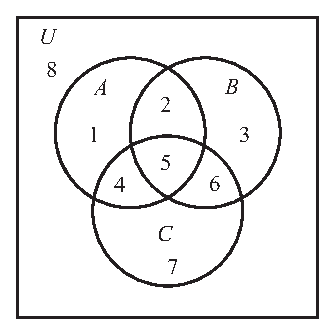
\includegraphics{figps-venn3.eps}
%\caption{Venn Diagram for Three Sets} \label{fig:venn3}
%\end{center}
%\end{figure}

In this diagram, there are eight distinct regions, and each region has a unique reference number.  For example, the set  $A$  is represented by the combination of regions 1, 2, 4, and 5, whereas the set  $C$  is represented by the combination of regions  4, 5, 6, and 7.  This means that the set $A \cap C$ is represented by the combination of regions  4  and  5.  This is shown as the shaded region in Figure~\ref{fig:aintersectc}.

\begin{figure}[h!]
\begin{center}
\scalebox{0.9}{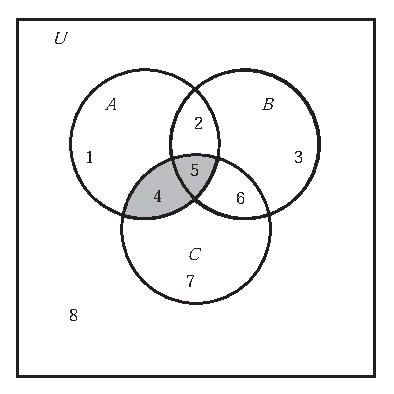
\includegraphics{figps-ainterc3.eps}}
\caption{Venn Diagram for $A \cap C$} \label{fig:aintersectc}
\end{center}
\end{figure}

Finally, Venn diagrams can also be used to illustrate special relationships between sets.  For example, if  $A \subseteq B$, then the circle representing  $A$  should be completely contained in the circle for  $B$.  So if  $A \subseteq B$, and we know nothing about any relationship between the set  $C$ and the sets $A$ and $B$, we could use the Venn diagram shown in Figure~\ref{fig:asubsetb}.

\begin{figure}[h!]
\begin{center}
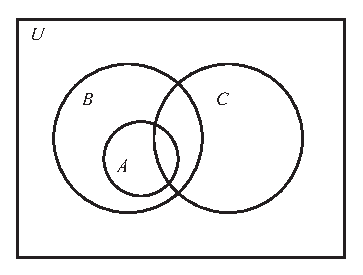
\includegraphics{figps-asubsetb3.eps}
\caption{Venn Diagram Showing $A \subseteq B$} \label{fig:asubsetb}
\end{center}
\end{figure}

\hbreak
\begin{prog}[\textbf{Using Venn Diagrams}] \label{prog:venndiagrams} \hfill \\
Let $A$, $B$, and $C$ be subsets of a universal set $U$.
\begin{enumerate}
  \item For each of the following, draw a Venn diagram for three sets and shade the region(s) that represent the specified set. 
  \begin{multicols}{2}
  \begin{enumerate}
   \item $(A \cap B) \cap C$
   \item $(A \cap B) \cup C$
   \item $\left( A^c \cup B \right)$
   \item $A^c \cap (B \cup C)$
  \end{enumerate}
  \end{multicols}
  \item Draw the most general Venn diagram showing $B \subseteq (A \cup C)$.
  \item Draw the most general Venn diagram showing $A \subseteq \left( B^c \cup C \right)$.
\end{enumerate}
\end{prog}
\hbreak



\endinput
 
